\documentclass[10pt,twocolumn]{article}
\usepackage[letterpaper,margin=0.78in,columnsep=0.27in]{geometry}
\usepackage[T1]{fontenc}
\usepackage{newtxtext,newtxmath}
\usepackage{microtype,booktabs,tabularx,amsmath,graphicx}
\usepackage{tikz}
\usetikzlibrary{arrows.meta,positioning}
\usepackage[hidelinks]{hyperref}
\hypersetup{pdftitle={Private LLM Inference: From Preparation to Decoding},pdfauthor={Blair Hudson},pdfsubject={Homomorphic preparation and complete private inference lifecycle}}
\usepackage{enumitem}
\setlist{nosep,leftmargin=*}
\setlength{\emergencystretch}{1.5em}
\setlength{\parskip}{2pt}
\title{Private LLM Inference:\\From Preparation to Decoding}
\author{Blair Hudson}
\date{6 September 2026}
\begin{document}
\maketitle
\begin{abstract}
Private language model inference must account for preparation, network transfer,
client computation and discarded work, not only the speed of a server kernel.
We study a protocol that prepares fresh additive masks with homomorphic
encryption and uses ordinary modular matrix multiplication during inference.
We complete a BFV coefficient matrix backend through ciphertext reconstruction
and client decryption. A matched 768 by 256 preparation stage becomes 4.93
times faster. We then execute complete dense stages at Qwen3.5 27B dimensions,
including a 5,120 by 34,816 expansion, and measure the full 248,320 row output
projection. A separate trained small decoder runs across isolated client and
server processes from an empty preparation inventory. Its generated tokens
match the clear quantized reference. Proposal verification reduces private
calls by 60 percent but is slower at low latency because rejected proposals
consume more preparation. Complete resource accounting for the 27B graph
identifies communication and client cryptography as primary constraints.
The work provides an executable inference trace and a capacity model; it does
not report generation from a loaded 27B checkpoint.
\end{abstract}

\section{Introduction}
A useful private inference system must answer the same questions as an ordinary
language model service: how soon does the first token arrive, how steadily do
later tokens arrive, and what resources does a conversation consume? Encryption
adds another question: can the service prepare cryptographic material faster
than inference consumes it?

PLLM separates the application interface from the private execution protocol.
An application can retain a Responses style interface, while a trusted client
component owns the prompt, tokenizer, cryptographic key and output decoding.
The remote service evaluates matrix operations without receiving their
unmasked inputs. This design makes conventional model matrices usable, but it
creates repeated interaction and preparation costs.

Our starting point packs many future masks into BFV plaintext coefficients.
Because the weights are small public integers, evaluating a linear map requires
only linear combinations of ciphertexts. A previous coefficient kernel computed
those combinations through integer matrix multiplication but did not complete
conversion back into ciphertext objects. We complete that path and then ask
whether its gains survive the complete inference lifecycle.

Three distinctions organize the evaluation. First, a prepared correlation is
one matrix input mask and its transformed output mask, not one language token.
A token may consume hundreds of correlations. Second, amortized throughput
from a large batch does not describe startup from an empty inventory. Third,
reducing network exchanges can increase preparation demand. A proposal that
is rejected still spent its cryptographic material.

The implementation contribution is a checked bridge between BFV objects and
integer coefficient matrices, a bounded evaluator for large matrix stages, and
an isolated execution harness that includes preparation replenishment. The
systems contribution is an accounting framework that exposes where improvements
move costs rather than remove them. We preserve dense integer matrices and do
not introduce a new model architecture or claim a new cryptosystem.

\section{Target graph and assumptions}
\subsection{A useful dense target}
We use the public configuration of Qwen3.5 27B as the large target
\cite{qwenconfig,qwencode}. Its text graph has width 5,120, 64 blocks and a
248,320 token vocabulary. Forty eight blocks use Gated DeltaNet; sixteen use
gated full attention. The feed forward width is 17,408. This is not an ordinary
attention only Transformer. Gated DeltaNet maintains a recurrent matrix state,
while the attention blocks maintain a growing key and value cache
\cite{gateddelta}.

We fuse projections only when they consume the same activation. The DeltaNet
input operation combines the query, key, value, output gate and two scalar
projections. Attention combines query, key and value, including the query output
gate. The two feed forward expansion matrices are also fused. The resulting
plan is in Table~\ref{tab:stages}.

\begin{table}[t]
\centering\small
\setlength{\tabcolsep}{4.5pt}
\begin{tabular}{lrrr}
\toprule
Stage & Input & Output & Count\\
\midrule
DeltaNet input & 5,120 & 16,480 & 48\\
Attention input & 5,120 & 14,336 & 16\\
Mixer output & 6,144 & 5,120 & 64\\
MLP expansion & 5,120 & 34,816 & 64\\
MLP contraction & 17,408 & 5,120 & 64\\
Vocabulary head & 5,120 & 248,320 & 1\\
\bottomrule
\end{tabular}
\caption{Public text execution plan for Qwen3.5 27B. The plan contains 257
private matrix exchanges per ordinary decode step. The embedding remains
local. These counts are derived from the configuration and source, not from an
executed full checkpoint.}
\label{tab:stages}
\end{table}

This plan includes 25.62 billion dense matrix elements. It excludes the vision
encoder, auxiliary prediction heads and a private embedding retrieval protocol.
The local embedding is a deliberate assumption, not a free operation: its
ideal four bit payload is 606.25 MiB, before scales, or 2.37 GiB at BF16.

\subsection{Security scope}
The weights are public. The service is assumed to follow the protocol while
observing its transcript. The client owns the BFV secret key, plaintext masks,
activation scales, recurrent state, attention cache and decoded output. The
server owns the dense matrices and public execution parameters. Table shapes,
message counts, timing and preparation schedules are observable.

The online messages contain no activation scale. A scale is derived from a
private activation and can itself disclose information. It is needed for
client dequantization, not the integer server operation. Uniform masks come
from operating system randomness with rejection sampling into the arithmetic
modulus. Deterministic generators are used only for public synthetic matrices
and training fixtures.

Transport authentication rejects altered or replayed frames. It does not prove
that a malicious provider applied the intended model. Standard HE
confidentiality is not a correctness guarantee, and arbitrary chosen layer
queries do not protect proprietary weights from a modified client. This study
does not extend its claim to either adversary. Hiding scheduling metadata and
handling restoration of a complete virtual machine snapshot also remain outside
the experiment.

\section{Protocol from preparation to output}
\subsection{The exact integer operation}
For a stage with integer matrix $W\in\mathbb Z^{m\times n}$ and activation $x$,
choose an arithmetic modulus $p$ and a fresh uniform mask $r\in\mathbb Z_p^n$.
During preparation the client sends $\operatorname{Enc}(r)$ and the server
computes $\operatorname{Enc}(Wr)$. The client decrypts and retains $(r,Wr)$.
During inference it sends $d=x+r\pmod p$, receives $u=Wd\pmod p$, and recovers
\begin{equation}
 u-Wr = W(x+r)-Wr = Wx \pmod p.
\end{equation}
The operation is exact in the ring. Recovering the corresponding signed dot
product additionally requires a sufficient range. For weights and activations
in $[-7,7]$, $p>98n$ is a conservative bound. We use $p=2,097,169$, which covers
the largest input width in Table~\ref{tab:stages}. This does not establish that
four bit activation quantization preserves the original floating checkpoint's
language quality.

For any fixed $x$, the online mask $x+r$ is uniform when $r$ is uniform. Reusing
a mask is different: subtracting two observed messages reveals
$x_1-x_2$. Every submitted row therefore consumes its correlation even if a
request fails or a proposed token is rejected. This restriction does not forbid
reusing an already decrypted result inside the client's own computation.

\begin{figure*}[t]
\centering
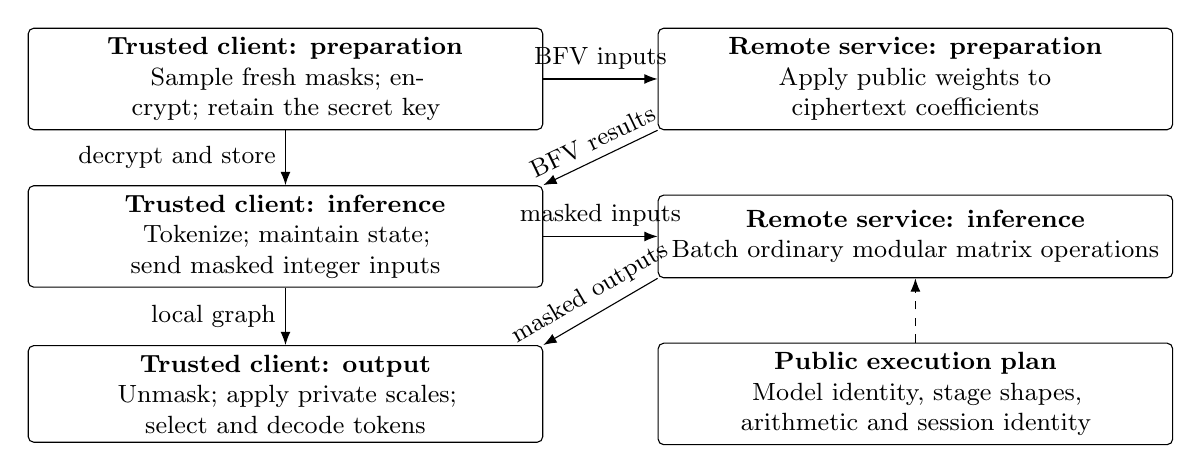
\begin{tikzpicture}[font=\small,box/.style={draw,rounded corners=2pt,align=center,text width=6.3cm,minimum height=1.05cm},>=Latex]
\node[box] (c1) at (0,0) {\textbf{Trusted client: preparation}\\Sample fresh masks; encrypt; retain the secret key};
\node[box] (s1) at (8,0) {\textbf{Remote service: preparation}\\Apply public weights to ciphertext coefficients};
\node[box] (c2) at (0,-2) {\textbf{Trusted client: inference}\\Tokenize; maintain state; send masked integer inputs};
\node[box] (s2) at (8,-2) {\textbf{Remote service: inference}\\Batch ordinary modular matrix operations};
\node[box] (c3) at (0,-4) {\textbf{Trusted client: output}\\Unmask; apply private scales; select and decode tokens};
\node[box] (s3) at (8,-4) {\textbf{Public execution plan}\\Model identity, stage shapes, arithmetic and session identity};
\draw[->] (c1.east) -- node[above]{BFV inputs} (s1.west);
\draw[->] (s1.south west) -- node[above,sloped]{BFV results} (c2.north east);
\draw[->] (c1.south) -- node[left]{decrypt and store} (c2.north);
\draw[->] (c2.east) -- node[above]{masked inputs} (s2.west);
\draw[->] (s2.south west) -- node[above,sloped]{masked outputs} (c3.north east);
\draw[->] (c2.south) -- node[left]{local graph} (c3.north);
\draw[->,dashed] (s3.north) -- (s2.south);
\end{tikzpicture}
\caption{Complete lifecycle. Preparation is included in the resource budget.
The fast online operation is masked modular arithmetic, not ciphertext only
inference. The client must remain within the customer's trusted environment.}
\label{fig:flow}
\end{figure*}

\subsection{Packing future masks by coordinate}
For $B$ future masks with $B\leq N$, encode coordinate $i$ as a polynomial
\begin{equation}
 P_i(X)=\sum_{b=0}^{B-1} r_{b,i}X^b.
\end{equation}
The server evaluates $Q_j=\sum_i W_{j,i}\operatorname{Enc}(P_i)$.
Coefficient $b$ of the decrypted result is exactly the $j$th coordinate of
$Wr_b\pmod p$. Scalar linear combinations never mix polynomial coefficients.
Thus the evaluator needs no rotations, rotation keys, bootstrapping, or products
of two ciphertexts. All masks packed together use the same encryption key.
Unrelated customer keys cannot be combined through ordinary batching.

BFV ciphertexts in this experiment contain two polynomials, one coefficient
prime $q$, and $N=2,048$ coefficients per polynomial. Writing their coefficients
as an $n$ by $2N$ residue matrix $A$ gives the server operation
\begin{equation}
 C=WA\pmod q.
\end{equation}
This is ordinary integer matrix multiplication on ciphertext representation,
not a change to BFV. We split residues into eight bit digits, convert each digit
to signed int8, apply an exact integer GEMM, and restore the public digit offset
with a row sum correction. Horner accumulation recombines the result modulo
$q$. The implementation checks int32 product bounds and uses int64 for modular
recombination. With $q<2^{54}$, the multiplication by 256 in this step remains
within the signed int64 range.

\subsection{Completing the library boundary}
Our bridge reads the documented SEAL serialization structure and reconstructs
ordinary ciphertexts that the SEAL loader validates. It accepts only the
measured representation: coefficient form BFV, two polynomials and one prime.
Linux anonymous memory files avoid persistent scratch files because the Python
binding accepts file paths. This is a checked research bridge, not a general
replacement for SEAL's native API.

Plaintext construction uses binary coefficient arrays rather than large
polynomial strings. Input digits are extracted through a byte view and retained
across output chunks. The evaluator produces bounded chunks rather than a full
large output coefficient matrix. Client decryption uses SEAL itself. These
changes retain the original integer weights and arithmetic.

\subsection{Consumption and local state}
A session receives a fresh epoch. A correlation identity binds a stage, batch
and row. The client reserves before sending, and the server marks identities
used before returning a result. Repeated identities and old epochs are rejected.
The demonstration discards remaining material at session close. It does not
claim that this policy survives restoration of a process and its entire memory.

Prompt prefill consumes a different mask for every prompt row. Attention,
normalization, activation functions and recurrent updates remain local. During
decoding, the client dequantizes each result with its retained activation scale
and public weight scales, then continues the graph. The output head is remote;
token selection and text decoding remain local. Figure~\ref{fig:flow} shows
where each phase executes.

\section{Experiments and implementation results}
\subsection{Method}
The environment exposes five logical CPUs, a quota of four CPU equivalents and
4 GiB of memory. It runs Python 3.13.5, PyTorch 2.10.0 and TenSEAL 0.3.17 on Linux.
No GPU is available. The large matrix experiments use synthetic public integer
weights at the verified target dimensions. No large model checkpoint is loaded.

The primary profile uses degree 2,048, plaintext modulus 2,097,169 and one 54 bit
coefficient prime. SEAL accepts the profile at its TC128 setting
\cite{seal,bfv}. Minimum observed invariant noise budgets are 18--21 bits on
large stages. Library validation and measured noise margins are not an
independent cryptographic audit.

There are three samples for the matched preparation comparison and two samples
for each full size preparation stage. Raw first use costs are retained. Online
matrix tests contain four samples, and the full vocabulary projection has three.
Large preparation checks compare all output columns against independent NumPy
integer arithmetic for 16 mask rows. Small tests compare every row. Coefficient
GEMM tests also compare with unbounded Python arithmetic and SEAL's own
ciphertext additions. Small differences between timings are not interpreted as
general hardware properties.

\subsection{Complete preparation}
Table~\ref{tab:prep} reports the complete path, including client encryption,
representation conversion, evaluation and client decryption. It excludes key
setup, reference checking and network transfer. The matched coordinate addition
control uses the same modulus, degree, weights and batch occupancy. At 768 to
256, its median 3.122 seconds becomes 0.633 seconds: a 4.93 times improvement.

\begin{table}[t]
\centering\small
\setlength{\tabcolsep}{4.5pt}
\begin{tabular}{lrr}
\toprule
Matrix stage & Batch time (s) & Correlations/s\\
\midrule
768 to 256, control & 3.122 & 656.1\\
768 to 256, complete GEMM & 0.633 & 3,235.3\\
5,120 to 16,480 & 16.56 & 123.7\\
5,120 to 14,336 & 15.24 & 134.4\\
6,144 to 5,120 & 8.39 & 244.2\\
5,120 to 34,816 & 32.26 & 63.5\\
17,408 to 5,120 & 19.03 & 107.6\\
\bottomrule
\end{tabular}
\caption{Actual BFV preparation with 2,048 future masks per stage. A correlation
is not a language token. All target size matrices contain synthetic W4 weights.}
\label{tab:prep}
\end{table}

The expansion spends 15.46 seconds in server GEMM, 2.35 seconds in client
encryption and export, and 13.82 seconds in client import and decryption. This
is no longer primarily a server kernel problem. The contraction shows a similar
shift: byte view extraction reduces digit preparation substantially, but client
encryption remains 8.80 seconds per batch.

We additionally test standard seeded symmetric encryption supported by SEAL.
The server expands the public seed representation before coefficient GEMM; it
never receives the secret key. Packing returned coefficients into seven bytes
is lossless because $q<2^{54}$. At 768 to 256, combined input and output traffic
falls 42.5 percent, from 33.55 MB to 19.31 MB. The complete local path is about
0.691 seconds, slightly slower than the raw representation. The choice is
therefore a bandwidth versus conversion trade, not an unconditional speedup.

\subsection{Online computation}
Invariant weight data and digit corrections are compiled once, not recomputed
for each request. We measure clear W4A4 integer GEMM and masked modular GEMM at
each target stage dimension. We also execute the complete 5,120 to 248,320
vocabulary projection rather than timing only its small tiles. Full head
correctness checks cover 128 output rows and every batch row using an
independent integer reference.

Summing measured stages with the counts in Table~\ref{tab:stages} gives
Table~\ref{tab:linear}. These are projections of matrix work, not full model
throughput. They omit attention, recurrence, lookup, transport and preparation.
Batch rows may represent concurrent sessions or candidate positions; aggregate
row rate must not be described as one user's output rate.

\begin{table}[t]
\centering\small
\setlength{\tabcolsep}{4.5pt}
\begin{tabular}{rrrr}
\toprule
Batch & Clear s/row & Masked s/row & Masked rows/s\\
\midrule
1 & 0.710 & 1.976 & 0.506\\
8 & 0.217 & 0.731 & 1.369\\
16 & 0.101 & 0.395 & 2.534\\
\bottomrule
\end{tabular}
\caption{Projected dense matrix work for the 27B text graph, summed from
measured stage shapes. These figures exclude all other inference costs.}
\label{tab:linear}
\end{table}

\subsection{More activation precision at small protocol cost}
A further arithmetic experiment keeps W4 weights but increases the activation
range to $[-127,127]$. A width 17,408 dot product with all weights equal to
$+7$ or $-7$ recovers the exact signed extrema $\pm15,475,712$. Using plaintext
modulus 33,554,467 and the same ciphertext profile retains a minimum observed
noise budget of 14 bits. The coefficient matrix program is unchanged.

Online residues now require four rather than three bytes. In the compact
27B accounting, this adds 6.32 MB per token, about 6.8 percent of combined
preparation and inference traffic. This is an arithmetic and communication
result for W4A8, not a measured improvement in model quality. It identifies a
compatibility experiment that need not pay for a different HE evaluator.

\section{The whole client and server lifecycle}
We train a four block, width 32 model containing three DeltaNet blocks and one
gated attention block, followed by a vocabulary head. The graph includes causal
convolution, partial rotary embeddings, RMS normalization and SwiGLU. It uses a
short authored text corpus, 160 ordinary next token optimization steps and
quantization during training. Its purpose is a functional learned checkpoint,
not competitive language quality.

The client and server are separate spawned processes. The server receives
public integer matrices and a transport authentication key, but no HE secret
key or plaintext mask. The client runtime contains a public embedding and small
normalization and convolution parameters, but no dense projection matrices.
All preparation uses actual BFV. There is no trusted dealer and no initial
inventory hidden from the timing.

The client processes an 18 token prompt and emits 96 tokens. Ordinary decoding
prepares 2,176 stage correlations, consumes 1,904 and leaves 272 unused.
The output trace includes a second preparation cycle after initial inventory
is exhausted. All generated tokens and final logits equal the clear W4A4
reference. A local run takes 2.90 seconds, including 2.01 seconds of preparation,
compared with 0.240 seconds for the clear graph. The first private token takes
1.09 seconds. These small model rates do not predict a 27B service.

\subsection{Fewer exchanges can still be slower}
We implement greedy proposal verification using continuations found in the
client's existing token history. It requires no second language model. The
target evaluates a fixed block of proposals, accepts a matching prefix and
returns the target correction or bonus token. This follows the established
principle of target verification, while prompt lookup is also available in
current inference libraries \cite{speculative,assisted}. We do not implement
the rejection sampling algorithm required for a general sampled distribution.

Every candidate row consumes fresh correlations. To recover accepted private
state, the client replays the accepted prefix using already decrypted matrix
outputs. It does not issue another matrix query. With four proposals, online
calls fall from 1,632 to 646, but consumed correlations rise from 1,904 to 3,434.
The workload is repetitive, so its proposal acceptance is not a general task
estimate.

\begin{table}[t]
\centering\small
\setlength{\tabcolsep}{4.5pt}
\begin{tabular}{rrrr}
\toprule
Added delay & Ordinary (s) & Proposals (s) & Speed ratio\\
\midrule
0 ms & 2.90 & 4.27 & 0.68\\
1 ms & 4.91 & 5.35 & 0.92\\
10 ms & 20.11 & 11.29 & 1.78\\
\bottomrule
\end{tabular}
\caption{Measured complete runs emitting 96 tokens from an empty preparation
inventory. Delay is injected once per online exchange; it is not a physical
wide area network measurement. Speed ratio is ordinary time divided by proposal
time. All runs produce the same token sequence.}
\label{tab:spec}
\end{table}

At low latency, the extra preparation exceeds the saved interaction time. At
10 ms per exchange, the interaction saving wins. An inference controller should
therefore minimize time per \emph{delivered} token, including rejected proposals,
not maximize proposed tokens per verification call. For $k$ proposals and
mean useful output $A_k$, a simple cost objective is
\begin{equation}
 T_k = \frac{L_{\rm exchange}+(k+1)C_{\rm row}+C_{\rm replay}}{A_k},
\end{equation}
where $C_{\rm row}$ includes preparation and transfer, not only GEMM. Acceptance
statistics should be measured by prefix, rather than assuming independent
acceptance events. The executable cost selector is an experiment utility; it
is not yet integrated into the public SDK's scheduler.

\subsection{Recurrent replay reduces memory}
The target's 48 DeltaNet layers use 144 MiB of FP32 recurrent state. Saving a
complete snapshot at each of eight proposal positions would add 1.125 GiB.
Saving query, key, value, decay and update traces instead uses 27.14 MiB, plus
the existing base state. Replaying four accepted positions takes 1.96 ms for
one real size layer in the measured implementation. The saved and replayed
prefix states match exactly when the same kernel and operation order are used.

A matrix kernel version of the recurrence is also checked against an elementwise
reference. Its maximum FP32 output difference is $3.34\times10^{-6}$; this is a
floating summation difference, not bit equivalence. Such differences must be
tested at quantization boundaries before deploying an existing checkpoint.
Recent TreeWY research independently removes speculative state snapshots through
structured reconstruction for Gated DeltaNet hybrids \cite{treewy}. Our simpler
sequential replay does not claim that contribution; it tests the value of
reconstructing state without another private query.

\section{Capacity at the 27B target}
\subsection{Preparation is not free inventory}
The public plan has 2,167,808 input values and 4,152,320 output values across one
decode step. With three byte residues, online transfer is 18.96 MB per token.
At full coordinate occupancy, two ciphertext polynomials stored as uint64
require 16 bytes per input or output coordinate per useful correlation.
Raw preparation therefore adds 101.12 MB per token set. The seeded input and
seven byte output experiment projects preparation at 74.63 MB per token set.

A one gigabit link shared between directions then has a 1.34 token/s bandwidth
ceiling for compact preparation plus inference. If each direction independently
supports one gigabit/s, the ceiling is 1.77 token/s. Both assume ideal overlap,
zero compute time and full batch utilization. The online only figure of 6.59
token/s ignores the larger preparation stream and is not a sustained bound.

The CPU preparation components sum to 2.49 seconds per complete token set.
For the head, output work is extrapolated from a measured 1,024 row tile;
common input work is counted once. Preparing 2,048 complete token sets projects
to 5,091 seconds of serial work on this host, before transport or online
inference. This is a capacity projection, not a full model timing.

\subsection{Memory and startup}
Keeping both uint32 masks for those 2,048 sets requires 48.22 GiB. Reproducible
input masks from a securely managed generator seed reduce input storage but
still leave 31.68 GiB of output masks. That is already larger than many client
machines, before model state or cryptographic working buffers.

At 8,192 positions, the sixteen full attention blocks require 512 MiB of BF16
KV state. The recurrent state adds 144 MiB and the convolution history adds
7.5 MiB. A zero weight client is not a zero resource client.

Prompt prefill offers a different scheduling opportunity. Its known token
rows can consume a stage's entire preparation batch immediately. Generating and
consuming one stage at a time bounds inventory memory. It does not remove the
work or communication. For short decode sessions, preparing thousands of future
rows improves an amortized rate while creating startup delay and unused stock.
A batch controller must account for its usable horizon.

\subsection{Interaction bounds and sparse models}
With 257 exchanges per token, 20 ms round trip latency alone adds 5.14 seconds
before arithmetic or transfer. A persistent socket avoids reconnection but does
not eliminate these data dependencies. Proposal verification can amortize some
exchanges, but additional rows increase preparation and bandwidth demand.

We also inspect Qwen3.5 35B-A3B \cite{moeconfig}. It selects eight of 256 experts.
Sending selected expert identifiers exposes a decision derived from private
state. Evaluating all experts multiplies expert work by 32 relative to the
selected set, before shared expert and attention work. A 3B active parameter
label therefore cannot be used as a private computation budget without a
separate private dispatch protocol. No such protocol is implemented here.

\section{Implications for the inference experience}
The application should retain a simple chat or Responses interface. The client
runtime should expose truthful local states: loading public assets, preparing,
processing the prompt, decoding, waiting for preparation, and finishing.
Useful telemetry includes time to first token, complete request time, output
spacing, preparation used and discarded, and bytes in each direction. Fast
output intervals between replenishment pauses should not be the headline rate.

A persistent customer agent can combine authorized sessions within the same
key and trust boundary, making preparation occupancy more predictable. This
is a deployment choice, not an instruction to move the client's keys onto an
untrusted provider. The measured resource plan is more compatible with a
customer gateway than an unassisted thin browser client.

The next priorities follow from the measurements. First, reduce preparation
communication using a reviewed matrix protocol. Work on silent correlation
generation motivates this direction \cite{silent}, but efficient scalar
correlations do not automatically provide a cheap arbitrary matrix product.
Second, complete a native batch bridge for client cryptography. Accelerating
only the remote GEMM leaves substantial client work unchanged. Third, compile
larger secure execution regions to reduce exchanges. Fourth, integrate bounded
inventory scheduling and proposal decisions into the existing SDK.

Finally, execute an actual Qwen checkpoint and compare quantized output quality
with its floating reference. The current large benchmarks preserve synthetic
integer matrices exactly; they do not establish existing checkpoint quality,
long context behavior or complete model throughput.

\section{Related work and conclusion}
BFV supplies the exact encrypted arithmetic used here \cite{bfv}. SEAL provides
its implementation and serialization \cite{seal}. Cheetah demonstrates the
importance of designing private linear protocols without expensive rotations
\cite{cheetah}. Our contribution is narrower: completion and evaluation of an
integer coefficient path, with the complete client lifecycle included.

Gated DeltaNet makes recurrent state a first class requirement for modern hybrid
models \cite{gateddelta}. Speculative decoding reduces serial target calls
\cite{speculative}, and state reconstruction can avoid large speculative
snapshots \cite{treewy}. Private inference adds an important qualification:
rejected work spends preparation that ordinary inference does not require.

The experiments support a practical conclusion. Preserving ordinary dense
integer matrices is compatible with much faster HE preparation, but preparation
throughput alone is not the user experience. At useful model dimensions,
communication, client cryptography, inventory horizon and sequential exchanges
must be optimized together. The supplied code makes these costs visible and
reproducible instead of hiding them behind an online kernel rate.

\section*{Reproducibility and limitations}
The artifact contains source, a UV project, a trained small Safetensors fixture,
raw timing samples, the public model plan and commands for each experiment.
The test suite checks exact modular arithmetic, ciphertext agreement, serialization,
state replay and transport replay rejection. Whole lifecycle measurements are
executed experiments, not claims of universal latency. The full target weights,
GPU execution, physical wide area networking, sampled speculative decoding,
private expert dispatch and malicious provider security are not evaluated.

\begin{thebibliography}{10}
\small
\bibitem{bfv} J. Fan and F. Vercauteren. Somewhat Practical Fully Homomorphic
Encryption. Cryptology ePrint 2012/144, 2012. \url{https://eprint.iacr.org/2012/144}.
\bibitem{seal} Microsoft Research. Microsoft SEAL. Library source and
serialization implementation, version 4.3.3.
\url{https://github.com/microsoft/SEAL}.
\bibitem{qwenconfig} Qwen Team. Qwen3.5-27B: model configuration and model card.
2026. \url{https://huggingface.co/Qwen/Qwen3.5-27B}.
\bibitem{qwencode} Hugging Face contributors. Qwen3.5 model implementation,
\texttt{modeling\_qwen3\_5.py}. Source inspected 6 September 2026.
\url{https://github.com/huggingface/transformers}.
\bibitem{gateddelta} S. Yang, J. Kautz and A. Hatamizadeh. Gated Delta Networks:
Improving Mamba2 with Delta Rule. ICLR 2025. \url{https://arxiv.org/abs/2412.06464}.
\bibitem{speculative} Y. Leviathan, M. Kalman and Y. Matias. Fast Inference from
Transformers via Speculative Decoding. ICML 2023.
\url{https://arxiv.org/abs/2211.17192}.
\bibitem{assisted} Hugging Face. Assisted decoding: speculative and prompt
lookup decoding. Transformers documentation.
\url{https://huggingface.co/docs/transformers/main/assisted_decoding}.
\bibitem{treewy} S. M. Ghantasala. TreeWY: Speculative Verification for Gated
DeltaNet Hybrids. arXiv:2608.20961, 2026.
\bibitem{moeconfig} Qwen Team. Qwen3.5-35B-A3B: model configuration. 2026.
\url{https://huggingface.co/Qwen/Qwen3.5-35B-A3B}.
\bibitem{silent} E. Boyle, G. Couteau, N. Gilboa, Y. Ishai, L. Kohl, P. Rindal
and P. Scholl. Efficient Two-Round OT Extension and Silent Non-Interactive
Secure Computation. Cryptology ePrint 2019/1159.
\url{https://eprint.iacr.org/2019/1159}.
\bibitem{cheetah} Z. Huang, W. Lu, C. Hong and J. Ding. Cheetah: Lean and Fast
Secure Two-Party Deep Neural Network Inference. USENIX Security 2022, pp. 809--826.
\end{thebibliography}
\end{document}
